\documentclass[letterpaper,10pt]{article}

% ==================== Packages ====================
\usepackage[empty]{fullpage}
\usepackage{titlesec}
\usepackage[dvipsnames,svgnames,x11names]{xcolor}
\usepackage{enumitem}
\usepackage{hyperref}
\usepackage{fancyhdr}
\usepackage{tabularx}
\usepackage{fontawesome5}
\usepackage{graphicx}
\usepackage{array}
\usepackage{geometry}
\usepackage{fontspec}
\usepackage{needspace}

% ==================== Page Settings ====================
\geometry{
    left=0.45in,
    right=0.45in,
    top=0.35in,
    bottom=0.38in,
    nohead
}

\pagestyle{fancy}
\fancyhf{}
\fancyfoot{}
\renewcommand{\headrulewidth}{0pt}
\renewcommand{\footrulewidth}{0pt}
\setlength{\footskip}{4.1pt}

\raggedbottom
\raggedright
\setlength{\tabcolsep}{0in}
\urlstyle{same}

% ==================== Colors ====================
\definecolor{link}{RGB}{34,78,160}
\definecolor{textgray}{RGB}{70,70,70}
\definecolor{lightgray}{RGB}{220,220,220}

\hypersetup{
    colorlinks=true,
    urlcolor=link,
    linkcolor=link,
    pdftitle={Zitao Xing Resume},
    pdfauthor={Zitao Xing}
}

% ==================== List Settings ====================
\setlist[itemize]{
    topsep=0.12em,
    itemsep=0.02em,
    parsep=0em,
    partopsep=0em,
    leftmargin=1.35pc
}

\renewcommand\labelitemi{\raisebox{0.2ex}{\tiny$\bullet$}}

% ==================== Custom Commands ====================
\newcommand{\SectionFont}{\fontsize{13.8pt}{15pt}\selectfont}

\titleformat{\section}{
    \vspace{-2pt}
    \color{link}
    \raggedright\SectionFont\bfseries
}{}{0em}{}[
    \vspace{-3pt}
    \color{link}\titlerule
    \vspace{-5pt}
]

\newcommand{\resumeSubheading}[4]{
    \vspace{2pt}
    \noindent
    \begin{tabularx}{\textwidth}{@{}X@{\hspace{1em}}r@{}}
        \textbf{#1} & \textbf{#2} \\
        \textit{\textcolor{textgray}{#3}} & \textcolor{textgray}{#4} \\
    \end{tabularx}
    \vspace{-4pt}
}

\newcommand{\resumeProject}[4]{
    \vspace{2pt}
    \noindent
    \begin{tabularx}{\textwidth}{@{}X@{\hspace{1em}}r@{}}
        \textbf{#1} & \textbf{#2} \\
        \textit{\textcolor{textgray}{#3}} & \textcolor{textgray}{#4} \\
    \end{tabularx}
    \vspace{-4pt}
}

\newcommand{\contactItem}[2]{
    \makebox[1.25em][c]{\textcolor{link}{#1}} \ #2
}

\newcommand{\skillItem}[2]{
    \noindent
    \begin{tabularx}{\textwidth}{@{}>{\raggedright\arraybackslash}p{3.7cm}@{\hspace{0.4cm}}X@{}}
        \textbf{#1} & #2
    \end{tabularx}
    \vspace{0.5pt}
}

% ==================== Document ====================
\begin{document}

% ==================== Header ====================
\vspace{1pt}

\begin{minipage}[c]{0.22\textwidth}
    \centering
    {\setlength{\fboxsep}{2pt}
    \fcolorbox{lightgray}{white}{
        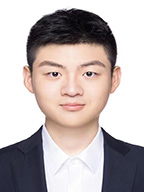
\includegraphics[width=3.0cm,height=3.6cm,keepaspectratio]{照片.jpg}
    }}
\end{minipage}
\hfill
\begin{minipage}[c]{0.74\textwidth}
    \raggedleft

    {\Huge \textbf{\textcolor{link}{Zitao Xing}}} \\[5pt]

    {\small
    \contactItem{\faIcon{map-marker-alt}}{Xiamen University, Xiamen, Fujian 361005, China} \\[3pt]
    \contactItem{\faIcon{phone}}{(+86) 18121271166} \\[3pt]
    \contactItem{\faIcon{envelope}}{\href{mailto:vincentxingzitao@gmail.com}{vincentxingzitao@gmail.com}} \\[3pt]
    \contactItem{\faIcon{github}}{\href{https://github.com/VincentXing23}{github.com/VincentXing23}} \\[3pt]
    \contactItem{\faIcon{globe}}{\href{https://zitao-xing-homepage.vercel.app}{zitao-xing-homepage.vercel.app}}
    }
\end{minipage}

\vspace{5pt}

% ==================== Education ====================
\section{Education}

\resumeSubheading
{Xiamen University}
{Xiamen, China}
{Incoming M.S. in Applied Mathematics (Operations Research), Recommendation-Based Admission}
{Sep. 2026}

\resumeSubheading
{Xiamen University}
{Xiamen, China}
{B.S. in Mathematics}
{Sep. 2022 -- Jun. 2026}

\resumeSubheading
{University of California San Diego}
{San Diego, CA, USA}
{University and Professional Studies (UPS) Program}
{Sep. 2024 -- Dec. 2024}

\vspace{1pt}
\noindent
\textbf{GPA}: 3.4/4.0
\quad
\textbf{Average Score}: 85/100
\quad
\textbf{Class Rank}: 16/49

% ==================== Internships ====================
\section{Internship Experience}

\resumeProject
{Shanghai Artificial Intelligence Research Institute}
{Shanghai, China}
{Algorithm Intern}
{Aug. 2026 -- Present}
\begin{itemize}
  \item Conduct research reproduction in AI for Science by reviewing problem formulations, methods, experimental settings, and evaluation protocols.
  \item Compare reproduced results with reported findings or baselines and document implementation choices, experimental observations, and remaining discrepancies.
\end{itemize}

\resumeProject
{\href{https://github.com/easyhang/evo_wiki}{Shanghai Big Data Co., Ltd. --- Evo Wiki}}
{Shanghai, China}
{Artificial Intelligence Development Intern}
{Jul. 2026 -- Aug. 2026}
\begin{itemize}
  \item Contributed to the development and improvement of Evo Wiki, an AI-native platform for maintainable Wiki and LightRAG workflows.
  \item Explored knowledge-graph extraction from legal materials and retrieval-augmented generation, focusing on entity-relation modeling, retrieval quality, and traceable evidence.
\end{itemize}

\resumeProject
{Harvest Fund Management Co., Ltd.}
{Shanghai, China}
{Shanghai Regional Office Intern}
{Jan. 2025 -- Mar. 2025}
\begin{itemize}
  \item Supported regional operations by organizing materials on fund products, market developments, client services, and institutional workflows.
  \item Used Excel and PowerPoint to consolidate, clean, format, and present market information, product materials, and peer-company data.
  \item Assisted with meeting preparation, client-document archiving, roadshows, and training materials, strengthening financial-data processing and cross-team communication skills.
\end{itemize}

% ==================== Research and Projects ====================
\section{Research \& Projects}

\resumeProject
{\href{https://github.com/Romanrose/shangtu-notebook}{Shanghai Library Open Data Competition --- Spatiotemporal Exploration Notebook}}
{Shanghai, China}
{Project Member}
{Aug. 2026}
\begin{itemize}
  \item Co-developed a touch-first PWA that lets users handwrite people, places, experiences, and works directly on a digital paper interface.
  \item Contributed to a workflow spanning handwriting transcription, constrained knowledge-graph retrieval, source-backed evidence verification, and traceable annotations.
\end{itemize}

\resumeProject
{\href{https://github.com/VincentXing23/Graphrag-for-Network/tree/main}{BGP-backed Network Digital Twin MVP with GraphRAG}}
{Personal Project}
{Developer}
{Jul. 2026 -- Present}
\begin{itemize}
  \item Built a network digital-twin MVP that transforms FRR-style BGP control-plane state into versioned snapshots and performs deterministic path lookup and before/after impact analysis.
  \item Implemented sample, FRR/containerlab live-lab, and synthetic scale modes; the scale scenario models 4 regions, 100 devices, and 12,000 route records per snapshot, with stale-data marking for partial collection failures.
  \item Integrated a GraphRAG layer using Neo4j graph persistence, Qdrant/vector fallback, and OpenAI-compatible or local LLM backends to provide evidence-grounded explanations.
  \item Exposed the system through Python CLI tools, a FastAPI service, Docker Compose, and a Cytoscape workbench that visualizes topology, path changes, collection status, and retrieval evidence.
\end{itemize}

\resumeProject
{Elite Undergraduate Summer Camp (EUSC $\times$ AISE), The Chinese University of Hong Kong, Shenzhen}
{Shenzhen, China}
{Participant}
{Jul. 2025 -- Aug. 2025}
\begin{itemize}
  \item Completed intensive training in deep learning and AI for Science, covering neural-network architectures, backpropagation, gradient-based optimization, loss design, model training, and evaluation.
  \item Built and trained a neural-network model, contributing to data preprocessing, architecture design, hyperparameter tuning, and experimental analysis from problem formulation through final presentation.
  \item Studied GPU parallel computing and CUDA fundamentals, and used Python and deep-learning frameworks to examine how hyperparameters affect convergence and generalization.
\end{itemize}

\resumeProject
{National-Level Research Training Project --- Functional Analysis Course GraphRAG}
{Xiamen, China}
{Project Leader}
{May 2025 -- May 2026}
\begin{itemize}
  \item Led a national-level undergraduate research project to build a knowledge-graph-enhanced retrieval system for a Functional Analysis course; coordinated project planning, technical integration, system validation, and presentation materials.
  \item Structured course resources into chapters, concepts, theorems, worked examples, and questions, and designed the relationships among these object types.
  \item Built a course knowledge graph containing 95 objects and 216 relationships to support hierarchical and associative organization of mathematical content.
  \item Developed a local GraphRAG demo with Neo4j, Qdrant, BAAI/bge-m3, BAAI/bge-reranker-v2-m3, and Flask, integrating semantic retrieval, vector recall, reranking, graph-context expansion, and pipeline visualization.
  \item Validated the end-to-end workflow from natural-language query to object retrieval, reranking, graph-context expansion, and evidence-chain display; explored integration with Alibaba Cloud agents and the Zhihuishu course platform.
\end{itemize}

\resumeProject
{Provincial Innovation Project --- Novel Numerical Methods for PDEs}
{Xiamen, China}
{Team Member}
{Apr. 2025 -- Apr. 2026}
\begin{itemize}
  \item Investigated numerical solutions of the Poisson equation on sector domains, focusing on how corner singularities and nonsmooth structures degrade conventional approximation accuracy.
  \item Helped design a Müntz-type basis method adapted to corner singularities and compared it with standard algebraic-power bases and a neural-network-assisted baseline.
  \item Conducted experiments on one-dimensional singular-function approximation, single- and double-mode Poisson benchmarks, and matched-versus-mismatched singular-exponent ablations; organized error data and visualizations.
\end{itemize}

% ==================== Honors ====================
\section{Honors \& Awards}

\begin{itemize}
    \item \textbf{2023 ``FLTRP ETIC Cup'' Understanding Contemporary China National Foreign Language Contest}, Provincial Second Prize
    \begin{itemize}
        \item Developed skills in English writing, logical argumentation, structured communication, and English-language research and presentation.
    \end{itemize}

    \item \textbf{2023 Contemporary Undergraduate Mathematical Contest in Modeling}, Provincial Third Prize
    \begin{itemize}
        \item Contributed to mathematical modeling, algorithm design, numerical experiments, and report writing in a team setting.
    \end{itemize}

    \item \textbf{AiXIA Innovation: Xiamen Hackathon, AI for Science / Agent Track}, Third Prize
    \begin{itemize}
        \item Contributed to SciVisualizer, a research agent that converts natural-language scientific intent into agent parsing, compute-task scheduling, visual rendering, and report generation.
        \item Helped refine the agent workflow across modeling, job submission, result parsing, and visualization, with emphasis on automation and clear user interaction for scientific computing.
        \item Applied mathematical and research-training experience to problem abstraction, scenario modeling, and pitch development, highlighting the workflow's potential to reduce tool fragmentation and improve research efficiency.
    \end{itemize}
\end{itemize}

% ==================== Skills ====================
\section{Skills \& Interests}

\skillItem{Programming}{Python, C/C++, MATLAB, CUDA}
\skillItem{Tools \& Platforms}{Git, VS Code, Alibaba Cloud}
\skillItem{Languages}{Chinese (native), English (proficient; IELTS 7.0)}
\skillItem{Research Interests}{Applied mathematics, machine learning, retrieval-augmented generation, operations research, graph algorithms, AI for Science, agent development}
\skillItem{Personal Interests}{Tea culture, coffee, badminton, long-distance running}

\end{document}
